\documentclass[11pt]{scrartcl}
\usepackage{graphicx}
\graphicspath{{./}}
\usepackage[sexy]{evan}
\usepackage[normalem]{ulem}
\usepackage{hyperref}
\usepackage{mathtools}
\hypersetup{
    colorlinks=true,
    linkcolor=blue,
    filecolor=magenta,      
    urlcolor=cyan,
    pdfpagemode=FullScreen,
    }
\usepackage[most]{tcolorbox}
\renewcommand{\dangle}{\measuredangle}

\renewcommand{\baselinestretch}{1.5}

\addtolength{\oddsidemargin}{-0.4in}
\addtolength{\evensidemargin}{-0.4in}
\addtolength{\textwidth}{0.8in}
% \addtolength{\topmargin}{-0.2in}
% \addtolength{\textheight}{1in} 


\setlength{\parindent}{0pt}

\usepackage{pgfplots}
\pgfplotsset{compat=1.15}
\usepackage{mathrsfs}
\usetikzlibrary{arrows}

\title{Session 4 - A week from battlefield}
\author{Azzam Labib (IG: haxuv.world)}
\date{G3-4 | 28 April 2024}
\begin{document}
\maketitle

\begin{enumerate}
    \section{Logical Thinking and Combinatorics}
    % \vspace{10cm} \item Among the 36 natural numbers from 1 to 36, at least how many numbers have to be picked so that there must be 2 numbers whose difference is 18?
    % \vspace{10cm} \item 6 different three-digit numbers can be formed using the digits "3", "6" and "8". Find the sum of these 6 three-digit numbers.
    
    \item Split the 4 numbers 6, 2, 0 and 9 into 2 groups and form 2 two-digit numbers respectively so that their product is maximized. Find the product.
    
    \vspace{10cm} \item The digit sum of each of several three-digit even numbers is 8, with no repeated digits. How many such three-digit even numbers are there?
    
    % \vspace{10cm} \item A Hacker enters the password "394052186" when he comes to the social media of someone. The system says they have swapped two of the numbers. How many passwords at most does the Hacker need to enter more?
    
    % \vspace{10cm} \item There are 55 cards. "1" is written on 1 card, "2" on 2 cards, "3" on 3 cards, \ldots, "10" on 10 cards. Now several cards are picked so that the sum of the numbers on all cards is 312. How many cards can be picked at most?
    
    \vspace{10cm} \item If $a \circ b = a + b + a \times b$, find the value of $5 \circ (8 \circ 3)$.
    % \vspace{10cm} \item If $a \diamond b = \begin{cases}
    %     2a + b & \text{if $a \geq b$} \\
    %     2b + a & \text{if $a < b$}
    % \end{cases}$, find the value of $(116 \diamond 16) \diamond (2 \diamond 8)$.
    % \vspace{10cm} \item Define the operation symbol $\oplus$ following this pattern:
    % \begin{align*}
    %     1 \oplus 5 &= 1 + 2 + 3 + 4 - 5\\
    %     3 \oplus 8 &= 3 + 4 + 5 + 6 + 7 - 8\\
    %     5 \oplus 9 &= 5 + 6 + 7 + 8 - 9\\
    %     \dots& \text{(and so on ...)}
    % \end{align*}
    % Find the value of $(5 \oplus 10) - (4 \oplus 9).$
    
    \vspace{10cm} \item Defined that the symbol $\triangle$ as an operation satisfies the following conditions:
    \begin{enumerate}[(i)]
        \vspace{10cm} \item When $a$ is odd, $a \triangle b = a \times 2 + b$,
        \vspace{10cm} \item When $a$ is even, $a \triangle b = a \div 2 + b$,
    \end{enumerate}
    evaluate $[(21 \triangle 12) \triangle 9] \triangle 3$.

    % \vspace{10cm} \item If $p \oplus q = p + 2 \times p + 3 \times q - 4 \times q + 5 \times p$, find the value of $3 \oplus 7$.

    % \vspace{10cm} \item Define $F(a)$ as $3 \times a+1$. Find the value of $n$ if $F(F(n))=40$.
    % \vspace{10cm} \item Defined that $a \otimes b \oplus c = a \times b + b \times c + c \times a$. Evaluate $8 \otimes 8 \oplus 8$.
    \vspace{10cm} 
    \section{Arithmetic/Algebra}
    \item Two brothers have 127 candies. The elder brother gives the younger brother half of his candies. The younger brother, after eating 16 candies, returns 24 candies to the elder brother. It ends up that the number of candies of the elder brother is twice of that of the younger brother. How many candies does the younger brother have in the beginning?
    % \vspace{10cm} \item 5 bags of rice, 6 bags of soybeans and 9 bags of red beans weigh 60 kilograms, while 17 bags of rice, 18 bags of soybean and 27 bags of red beans weigh 200 kilograms. So how many kilograms does 1 bag of rice weigh?
    % \vspace{10cm} \item Ronny runs after Sunny at a speed of 25 km/h. In the beginning, Sunny is 3 km ahead of Ronny. If Ronny manages to meet Sunny 12 minutes later, how many kilometres does Sunny run each hour?
    % \vspace{10cm} \item The ages of Mickey and Chesney add up to 95. The age of Mickey is 25 more than 4 times that of Chesney. Find the age of Mickey.
    % \vspace{10cm} \item There are two positive integers. Their sum is 143 and their product is 1080. Find the greater number among these two numbers.
    \vspace{10cm} \item For an arithmetic sequence of more than 10 terms, each term is added by the same number. It ends up that the sum of the arithmetic sequence is increased by 111. Find the sum of all possible values of the number of terms.
    % \vspace{10cm} \item There are 352 passengers on the train in the beginning. Upon arrival at the station, 175 passengers get off and 169 passengers get on. How many passengers are there on the train now?
    % \vspace{10cm} \item The number $20170312201703122017\ldots$ is written on and on. What is the $90^{th}$ digit?
    \vspace{10cm} \item Yolanda is 4 years older than her younger brother. Her father is 5 years younger than her mother. Yolanda's mother is now 40 years old. The age of Yolanda's father is 5 times that of Yolanda. How many years old is Yolanda's younger brother?
    \vspace{10cm} \item A restaurant spends 540 dollars to buy 20 cups and 20 plates. A cup costs 3 dollars more than a plate. How much is a plate?
    % \vspace{10cm} \item 42 trees are planted along a road from one end to another on both sides. Every two adjacent trees are 8 metres apart. How long is the road in metres?
    \vspace{10cm} \item 2 lawn mowers can clear a lawn of 80 square metres in 5 hours. At such rate, how many hours does it take for 5 lawn mowers to clear a lawn of 400 square metres?
    % \vspace{10cm} \item The four members in Mandy's family have their ages add up to 99. Her brother is 8 years younger than Mandy. Dad is 3 years older than Mum. 10 years ago, the family ages added up to 65. How old is Mum this year?
    \vspace{10cm} \item Evaluate $2024^2-2023^2$.
    \vspace{10cm} \item Evaluate $(23 \times 17 + 9) \div (12 \times 8 + 4).$
    % \vspace{10cm} \item Evaluate the value of $3 \times (2024^2 - 2^2) \div (2022 \times 2026)$.
    % \vspace{10cm} \item Evaluate $20^2-18^2+16^2-14^2+\dots+4^2-2^2$.
    \vspace{10cm} \item Evaluate $\dfrac{1}{1 \times 2} + \dfrac{1}{2 \times 3} + \dfrac{1}{3 \times 4} + \dots + \dfrac{1}{9 \times 10}$.

    \vspace{10cm} 
    \section{Number Theory}
    % \vspace{10cm} \item Find the number of positive factors of 35.
    % \vspace{10cm} \item Find the sum of all positive factors of 35.
    \item If the sum of two positive integers is 22, how many combinations of these two numbers are there? ($1$ and $21$ are counted as 1 combination only)
    % \vspace{10cm} \item Find the remainder when $19 \times 20 \times 21$ is divided by 9.
    \vspace{10cm} \item A 7-digit number $2017\,4AA$ is divisible by 12. Find the sum of possibilities of A.
    \vspace{10cm} \item If a number is divisible by 26, find the largest possible value of the remainder when that number is divided by 91.
    \vspace{10cm} \item Find the value of the following expression: \\
        $111111111 \div 111$
    % \vspace{10cm} \item Find the units digit of \\
    %     $88 \text{ "3"'s}$
    % \vspace{10cm} \item Find the remainder when $2017\,2017\,2017\ldots2017$ (with 2017 "2017"'s) is divided by 9.
    % \vspace{10cm} \item In the calculation below, the divisor and the quotient are equal. What is the least value of the dividend? \\
    %     $\square \div 12 = 12$
    \vspace{10cm} \item In a multiplication of two numbers, the units digit 4 in one of the numbers is mistakenly written as 9 and as a result the product acquired is 722. If the correct product is 532, find the larger number.

    \newpage
    \section{Geometry}
    \item The shaded part is a square. How many centimetres is the perimeter of the largest rectangle?
    \begin{figure}[h]
        \centering
        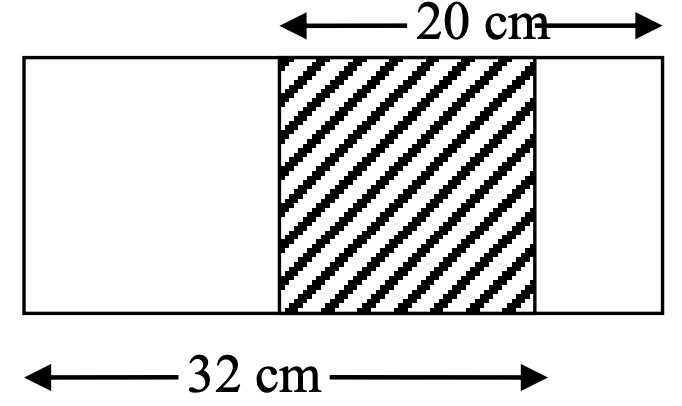
\includegraphics[width=0.4\textwidth]{StarGen/AIMO Trial G3-4 2024/shaded-square.png}
    \end{figure}
    
    % \vspace{10cm} \item The figure shows some numbered squares. If squares are to be tiled up to 2024 following the pattern, find the number in the square which is just above 127. 
    % \begin{figure}[h]
    %     \centering
    %     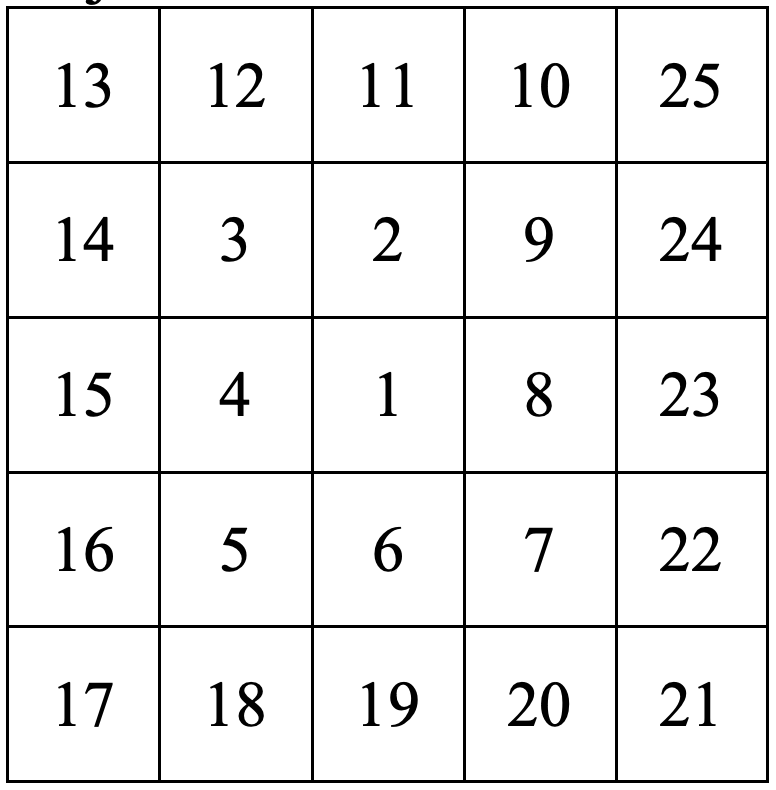
\includegraphics[width=0.4\textwidth]{StarGen/AIMO Trial G3-4 2024/square-siput.png}
    % \end{figure}
    
    \vspace{10cm} \item The figure is formed by several squares of different sizes, where the numbers stand for their areas. Find the perimeter of the figure.
    \begin{figure}[h]
        \centering
        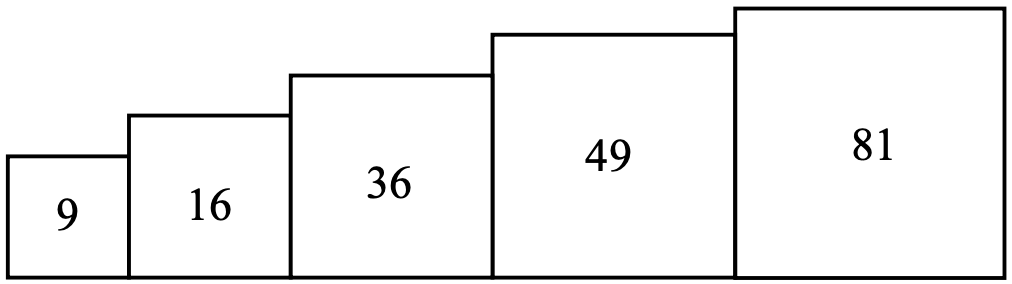
\includegraphics[width=0.4\textwidth]{StarGen/AIMO Trial G3-4 2024/several-square.png}
    \end{figure}
    
    \vspace{10cm} \item In the figure, $ABCD$ is a rectangle. The lengths of AE, $EF, FG, GH, HI, IJ$ and $JC$ are 20, 22, 24, 26, 28, 30 and 32 centimetres respectively. What is the difference between the areas of octagon $AEFGHIJD$ and $BEFGHIJC$ in square centimetres?
    \begin{figure}[h]
        \centering
        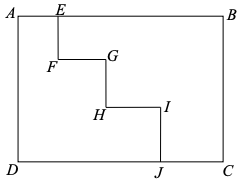
\includegraphics[width=0.4\textwidth]{StarGen/AIMO Trial G3-4 2024/octagon.png}
    \end{figure}
\end{enumerate}

\end{document}